\documentclass[
../../Software_Engineering_Summary.tex,
]
{subfiles}

\externaldocument[ext:]{../../Software_Engineering_Summary.tex}
% Set Graphics Path, so pictures load correctly
\graphicspath{{../../}}

\begin{document}
\subsection{Responsibility-Driven Design}
\begin{defbox*}
    Describes a systematic approach to think about the design of software objects and components in terms of \defc{responsibilities}, \defc{roles} and \defc{collaborations}.
\end{defbox*}

\subsubsection{Responsibility Types}
Responsibilities in general are related to
\begin{itemize}
    \item \defc{Obligations} of an object
    \item \defc{Behaviour} of an object
\end{itemize}
in terms of its role in the software design.

\begin{defbox}
    [Type: Doing Responsibility]
    Doing Responsibilities describe responsibilities that are related to performing a task.
    \begin{itemize}
        \item Doing it (perform a calculation, create an object)
        \item Initiate action in other objects
        \item Control and coordinate activities in other objects
    \end{itemize}
    For Example: A Bill object is responsible for calculating the total price.
\end{defbox}

\begin{defbox}
    [Type: Knowing Responsibility]
    Knowing Responsibilities describe Responsibilities that are related to \defc{knowing} and \defc{providing} information to other objects.
    \begin{itemize}
        \item Knowing private, encapsulated data
        \item Knowing related objects
    \end{itemize}
    For Example: A Car is responsible for knowing the driven distance.
\end{defbox}

\subsubsection{Responsibilities and Methods}
A responsibility is \defc{NOT} the same as a method. A responsibility can be modelled with a method, but in many cases its better to model it with multiple. Therefore a method is part of a responsibility and can be the whole responsibility, but a responsibility can also be split into multiple methods.

There is no real method to determining how to split responsibilities. It is often very circumstancial and needs to be adjusted to the needs at hand.

\subsection{More Design Principles}
Ideally a system design should follow the \defc{Single Responsibility Principle (SRP)}. This means that a class / object should have a responsibility which is its primary reason to change. Therefore one responsiblity per class is the ideal.

\subsubsection{Collaboration of Multiple Classes}
Oftentimes a oolicy requires collaboration of multiple classes. This makes it hard to choose which of these classes should handle the responsibility. There is also no easy answer for this. Sometimes there is a clear class that makes access to the others easier. To figure this out multiple drafts may be needed.

\subsubsection{Delegation vs. Inheritance}
To figure out where to place specific responsibilities the concepts of delegation and inheritance are useful. 

\begin{defbox}
    [Delegation]
    Delegates responsibilities to other objects:
    \begin{itemize}
        \item Get objects from other class with the needed functionality
        \item Use the object to fulfil only the needed functionality
        \item Inheritance hierarchy remains unchanged
    \end{itemize}
\end{defbox}

\begin{defbox}
    [Inheritance]
    Inherit responsibilities from baseclass:
    \begin{itemize}
        \item Violates SRP
        \item All subclasses of the current class are forced to also inherit the responsibility
        \item Not required functionality from the baseclass is also inherited
        \item Inheritance hierarchy is changed \rightarrow harder to maintain and understand
    \end{itemize}
\end{defbox}

Most of the time delegation is preferred. As the design is more understandable and maintainable. It also is evaluated at runtime rather than compiletime.  Inheritance should only be used when the responsiblity extends the functionality \defc{organically}.

\subsection{Encapsulation}

\begin{defbox}
    [Interface]
    An Interface declares the method signatures and public constants of its implementing classes. They provide independence of functionality from implementation.
\end{defbox}

\begin{defbox}
    [Always Program to Interfaces]
    \begin{itemize}
        \item Fields, return types, method parameters etc. should be declared with interface type
        \item Public methods should not expose implementation details
        \item Fields in implementing classes should be private. Retrieval \& modification of information via getters and setters should be used.
    \end{itemize}
\end{defbox}

This process has the advantages:
\begin{itemize}
    \item Avoids unjustified assumptions about implementation
    \item Interfaces are more stable than implementations
    \item To change the implementation its sufficient to exchange the constructor
    \begin{itemize}
        \item Can factor out implementation-independent code into abstract classes
        \item Reduces coupling
    \end{itemize}
\end{itemize}

\subsubsection{Field Access}
Instance fields should \defc{NEVER} be public. This ensures that information is hidden and adheares to the "Always Program to Interfaces" rule. 

It also makes sure that there is a distinction between implementation-specific data and public data. Client should not be able to access implementation-specific data.

\subsubsection{Accessor Methods Should not Expose More Than Necessary}
\begin{figure}
    [htp]
    \centering
    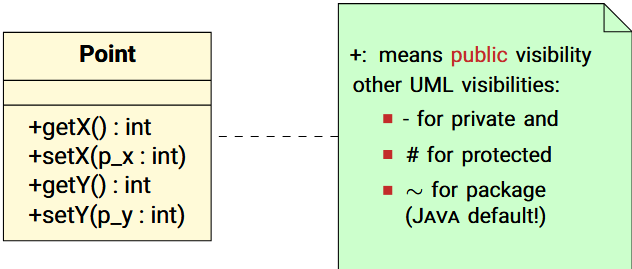
\includegraphics[width = 0.55\textwidth]{Pics/07/UMLAccessModifiers.png}
    \caption{UML Access Modifiers}
\end{figure}

Accessors shouldn't always be used. Oftentimes the use of accessors is unnecessary and only creates more coupling. In many cases it's better to outsource the responsibility of the accessor / the surrounding responsibility to another class instead.

There are some reasons to use accessors though:
\begin{itemize}
    \item Responsible for aspects of the UI (Data important for visualization)
    \item Class using accessors implements a policy
    \item Class is a static container
\end{itemize}

\subsection{Design Knowledge: The God Class Problem}

\begin{defbox}
    [God Class]
    A class that contains most of the system logic:
    \begin{itemize}
        \item Promotes poorly distributed responsibilities
        \item Not object oriented design
    \end{itemize}
\end{defbox}

To avoid this you can use the following criteria:
\begin{itemize}
    \item Avoid classes with unclear responsibilities
    \begin{itemize}
        \item Classes that fail the SRP principle
        \item Solution: Split class and relocate the responsibilities
    \end{itemize}
    \item Avoid classes with low cohesion and non-communicating classes
    \begin{itemize}
        \item Classes with methods operating on a small subsets of its fields but not with other objects
        \item Solution: Split class and relocate the responsibilities
    \end{itemize}
    \item Avoid classes with public field accessors:
    \begin{itemize}
        \item Public field accessors can indicate wrongly located responsibilities
        \item Solution: Redesign interface and relocate the responsibilities
    \end{itemize}
\end{itemize}

In general, when designing a system, one should try to model the real world. This however can produce complex systems. Therefore often it is advised to put the real world model aside and design the system as according to the design principles.
\end{document}